\chapter{Dynamic Active Curricula}\label{ch:DAC}
The results laid out in Chapter \ref{ch:BootstrappedActiveCurricula} suggest that generalisation performance can indeed be improved through the use of a learning curriculum, and that using active learning approaches to score which training samples are hard or difficult can be an effective way of automatically constructing such curricula without manually analysing the training samples. The disadvantage with the BAC method from Chapter \ref{ch:BootstrappedActiveCurricula} however is that it is necessary to first train a `baseline' model that can be used to derive a curriculum based on which samples it is uncertain about classifying. While in some cases this may not too significant a computational burden, it does effectively double the overall training time, motivating the approach laid out in this section. Specifically, we wish to investigate methods that can dynamically construct a curriculum throughout training, without needed to reference another model. We do this by calculating the model uncertainty on the training samples throughout training, using the uncertainty scores to construct dynamic curricula which evolve throughout training to focus on the samples that the model is more, or less, uncertain in its predictions. If succesful, these methods should lead to model performance which beats a the benchmark test set performance of a baseline model trained with normal mini-batch stochastic gradient descent on the entire training set, and hopefully will achieve results similar to those achieved by the bootstrapped active curricula from Chapter \ref{ch:BootstrappedActiveCurricula}.
\section{Curriculum Construction}
\subsection{Dynamic Task Curricula (DTC)}\label{sec:DTC}
The first dynamic curriculum method we test we term \textit{dynamic task curricula}; this approach is very similar to that of the BAC method laids out in Chapter \ref{ch:BootstrappedActiveCurricula}, however instead of constructing tasks based on the uncertainty scores of a fully trained baseline model, tasks are constructed dynamically using the uncertainty of the curriculum model itself throughout training. To do this, we calculate the model's uncertainty in predicting the classes of the training samples in the full training set $\mathcal{T}$ using the AADT function \ref{BAC_AADT} (or another active learning uncertainty measure) at the end of every epoch, then ranking the training sample by the the model's uncertainty. We then split the training data into separate tasks, with the first task consisting of the first $\frac{1}{T}$ samples where $T$ is the chosen number of tasks. At the start of each epoch, we will obtain a new set of ordered tasks, $\mathcal{T}_i^1, \mathcal{T}_i^2,...,\mathcal{T}_i^T$, where $i$ is the current epoch, and $T$ is the chosen number of tasks. Training is divided into $T$ phases, such that, during epoch $i$ of phase $t$, the model is trained on a training set consisting $\mathcal{T}_i^1 \cup \mathcal{T}_i^2 \cup ... \cup \mathcal{T}_j^t$, where $t$ denotes the current training phase.The final training phase will therefore consist of training on the full training set, as $\mathcal{T} = \mathcal{T}_i^1 \cup \mathcal{T}_i^2 \cup ... \cup \mathcal{T}_i^T, \forall  i$. As in the BAC curriculum method \ref{ch:BootstrappedActiveCurricula}, we normalise the number of parameter updates in each phase by scaling the number of epochs relative to the number of samples in the training set for that phase. Similarly in Equation \ref{eq:BAC_Epochs}, the number of epochs in training phase $t$ is set as follows:
\begin{equation}\label{eq:DTC_Epochs}
NumEpochs^{t} =\floor{ \frac{TotalEpochs}{t}}
\end{equation}
where $TotalEpochs$ is the number of epochs the model would need to be trained for on the whole training set in order to achieve the same number of parameter updates as the DTC curriculum method.

Note that we can rank the samples from low to high uncertainty or from high to low uncertainty; in the low to high case the first tasks will contain samples about which the model is confident in predicting, corresponding to dynamically constructing an easy to hard curriculum. Alternatively, ranking the samples from high to low uncertainty will produce a curriculum more similar to an active learning approach, focussing on training the model on areas of the input space that it is more uncertain about classifying. While the latter method may contradict some of the underlying motivations for curriculum learning, for example that learning with an easy to hard curriculum allows the model to explore a smoother version of the error space and better initialise the parameters, we would still argue that the hard to easy approach still qualifies as a curriculum method, and may be appropriate in instances where the model already has achieved a high level of expertise in the problem, and improvements are therefore more likely to be made by studying harder samples than easy ones.  We therefore have two variations of the Dynamic Task Curriculum method; Easy to Hard DTC and Hard to Easy DTC. This approach is similar to that of \textit{Self-Paced Learning} REF KOLLER ET AL, where they apply a similar approach with a latent SSVM model REF, however they implement their method by introducing a regularization term reflecting the difficulty of each sample into the objective function of the model, as opposed to employing an actual curriculum. As the model parameters are initialised randomly, it would be inappropriate to infer model uncertainty before the first epoch, as such, the first epoch is trained using the whole training set, and the use of the curriculum method begins starting with the second epoch.  Pseudocode for the DTC method is given in section \ref{sec:DTCPseudocode}.

\subsubsection{Pseudocode for the DTC curriculum}\label{sec:DTCPseudocode}
Pseudocode for the dynamic task curriculum method (assuming the use of the AADT uncertainty function and an easy to hard curriculum):
\begin{algorithmic}
\FOR {$i=1$ to $Num\_Epochs$}
\STATE $TrainingPhase = \floor{\frac{i*Num\_Tasks}{Num\_Epochs}}$
\STATE $PhaseEpochScale = \frac{Num\_Tasks}{TrainingPhase}$
\FOR {$PhaseEpochScale$}
\STATE $\mathbf{S}^{\theta_{curriculum}} = AADT_{\theta_{curriculum}}(\mathcal{T})$
\STATE $\mathcal{T}_{\mathbf{S}^{\theta_{curriculum}}} = \mathcal{T}, \text{sorted by } \mathbf{S}^{\theta_{curriculum}} \text{ (descending order)}$ 
\STATE $Num\_Samples = |\mathcal{T}_{\mathbf{S}^{\theta_{baseline}}}|$
\FOR {$t=0$ to $Num\_Tasks$}
\STATE $TaskStartIndex = Num\_Samples*\frac{t}{Num\_Tasks} $
\STATE $TaskEndIndex = Num\_Samples*\frac{t+1}{Num\_Tasks} $
\STATE $\mathcal{T}^{t}_{\mathbf{S}^{\theta_{baseline}}} = \mathcal{T}_{\mathbf{S}^{\theta_{baseline}}}[TaskStartIndex:TaskEndIndex,:] $
\ENDFOR
\STATE $\text{train }  \theta_{curriculum} \text{ on training set } \mathcal{T}^{0:TrainingPhase}_{\mathbf{S}^{\theta_{baseline}}} $
\ENDFOR
\ENDFOR
\end{algorithmic}


\subsection{Dynamic Sampling Curricula (DSC)}
The second dynamic curriculum construction method we test is \textit{Dynamic Sampling Curricula (DSC)}; one of the potential problems with some curriculum and active learning methods is that of \textit{diversity} REF PAPER ON DIVERSITY. Diversity refers to how well the whole training set is represented in the samples used to train the model; if a sample selection method is extremely undiverse then it may end up selecting only a very small selection of the training samples, leading to the model not training on a suitably broad set of training samples, resulting in high generalization error. One way to approach this problem is to avoid deterministic methods of selecting training examples, and instead sample from the training data using some probability distribution. Mini-batch stochastic gradient descent REF? is one such method, sampling batches of examples from the training data using a uniform probability distribution, however by varying the sampling distribution away from a uniform distribution we can bias training towards different samples, resulting in them being selected more or less often than others. 

We implement the DSC curriculum method by biasing the sampling probability proportionally to the model uncertainty in predicting the labels of the sample. In particular, at the start of every epoch we use an uncertainty function (for example the AADT function introduced in \ref{BAC_AADT}) to infer the model's current uncertainty in predicting the labels of the training data, giving $\mathbf{S}^{\theta_{baseline}}$, a vector of $N$ scores as in Equation \ref{eq:BAC_S}, where the $N$ is the number of samples in the full training set $\mathcal{T}$ and the $i^{th}$ element of $\mathbf{S}$ corresponds to the ouput of the AADT function for the $i^{th}$ training input. We then pass the vector of scores through a softmax function, effectively transforming the scores into probabilities that can be used as the sampling probability function (defined assuming the uncertainty function used is the AADT function):
\begin{equation}\label{eq:DSC_Prob}
\tilde{p_j}(x_i | \theta_j) = \frac{exp(\frac{AADT_{\theta_j}(x_i)}{\tau})}{\sum_{k}^{N} exp(\frac{AADT_{\theta_j}(x_k)}{\tau})}
\end{equation}
where $\theta_j$ is the model being trained with the curriculum after $j-1$ epochs, $\tilde{p_j}(x_i | \theta)$ is the sampling probability of training sample $i$ in the $j^{th}$ training epoch, and $\tau$ is the softmax temperature parameter that can be set as a hyperparameter or tuned each epoch to achieve a target diversity level in the sampling probability. The sampling probability is updated at the start of each epoch and training proceeds as with uniform mini-batch stochastic gradient descent, using the sampling probabilities calculated in Equation \ref{eq:DSC_Prob}. As we wish to bias training towards certain certain/uncertain samples, we also do not follow the typical SGD practice of sampling without replacement, instead sampling with replacement. As sampling with replacement implies that some samples will probably not be used in every epoch, this in effect introduces a stochastic curriculum where, instead of removing samples entirely from certain training phases, we instead decrease their probability of being sampled during an epoch. Unlike the DTC curriculum method in Section \ref{sec:DTC}, the DSC method does not have distinct training phases; the sampling probability is biased throughout the entirety of training. As we are no longer using training phases with smaller task training sets we do not need to modify the number of epochs relative to the baseline as we did with the BAC method in Chatper \ref{ch:BootstrappedActiveCurricula} and the DTC method. As with the DTC method in the previous section, we train the model using the whole training set, with uniform mini-batch SGD, for one epoch, before we begin estimating model uncertainty and training with the DSC curriculum. Pseudocode for the DSC curriculum method is given in Section \ref{sec:DSCPseudocode}.

\subsubsection{Pseudocode for the DSC curriculum}\label{sec:DSCPseudocode}
Pseudocode for the dynamic sampling curriculum method, except for the softmax temperature control method, given in REF (assuming the use of the AADT uncertainty function and an easy to hard curriculum):
\begin{algorithmic}
\FOR {$j=1$ to $Num\_Epochs$}
\STATE $\forall x_i \in \mathcal{T}, \tilde{p_j}(x_i | \theta_j) = \frac{exp(\frac{AADT_{\theta_j}(x_i)}{\tau})}{\sum_{k}^{N} exp(\frac{AADT_{\theta_j}(x_k)}{\tau})}$
\STATE $\text{train }  \theta_{curriculum} \text{ on training set } \mathcal{T}, \text{ sampled with probabilities }  \tilde{p}(. | \theta_j)  $
\ENDFOR
\end{algorithmic}

\subsection{Dynamic Sampled Task Curricula (DSTC)}
The final dynamic curriculum method implemented combines the the DTC and DSC methodologies, into an approach we term \textit{dynamic sampled task curricula (DSTC)}. As in the dynamic task curricula method, at the start of every epoch we calculate the model uncertainty on the samples in the training set  $\mathcal{T}$, dividing the training set up into several equally sized tasks of increasing or decreasing uncertainty. Again as in the DTC approach, the model is trained in several phases; in the first phase only the first task is using to train the model, then in the second phase the first two tasks are used, and so on until the entirety of $\mathcal{T}$ is being used. In the DSTC approach however, instead of sampling uniformly from training samples used in each phase, we bias the sampling probability as in the DSC model. We therefore calculate the sampling probability for sample $x_i$ in epoch $j$ as follows, assuming $j$ falls in phase $t$:

\begin{equation}\label{eq:DSC_Prob}
\tilde{p_j}(x_i | \theta_j) = 
\begin{cases} 
\frac{exp(\frac{AADT_{\theta_j}(x_i)}{\tau})}{\sum_{k}^{K} exp(\frac{AADT_{\theta_j}(x_k)}{\tau})} & \text{if } x_i \in \mathcal{T}_j^1 \cup \mathcal{T}_j^2 \cup ... \cup \mathcal{T}_j^t \\
0 & \text{if } x_i  \notin \mathcal{T}_j^1 \cup \mathcal{T}_j^2 \cup ... \cup \mathcal{T}_j^t
\end{cases}
\end{equation}
where $K$ is the number of training samples in the phase training set $\mathcal{T}_j^1 \cup \mathcal{T}_j^2 \cup ... \cup \mathcal{T}_j^t$, (assuming we are using the AADT uncertainty function to estimate model uncertainty).

The DSTC method therefore combines the DTC and DSC methods, dynamically splitting the training data into uncertainty based tasks, and then sampling from the tasks proportionally to the uncertainty of the samples relative to the rest of the task. DSTC could therefore be considered a more general version of the DSC method, where the DSC method is simply a special case of DSTC, where the number of tasks is equal to one. Pseudocode for the DSTC method is given in the following section.

\subsubsection{Pseudocode for the DSTC curriculum}\label{sec:DSTCPseudocode}
\begin{algorithmic}
\FOR {$i=1$ to $Num\_Epochs$}
\STATE $TrainingPhase = \floor{\frac{i*Num\_Tasks}{Num\_Epochs}}$
\STATE $PhaseEpochScale = \frac{Num\_Tasks}{TrainingPhase}$
\FOR {$PhaseEpochScale$}
\STATE $\mathbf{S}^{\theta_{curriculum}} = AADT_{\theta_{curriculum}}(\mathcal{T})$
\STATE $\mathcal{T}_{\mathbf{S}^{\theta_{curriculum}}} = \mathcal{T}, \text{sorted by } \mathbf{S}^{\theta_{curriculum}} \text{ (descending order)}$ 
\STATE $Num\_Samples = |\mathcal{T}_{\mathbf{S}^{\theta_{baseline}}}|$
\FOR {$t=0$ to $Num\_Tasks$}
\STATE $TaskStartIndex = Num\_Samples*\frac{t}{Num\_Tasks} $
\STATE $TaskEndIndex = Num\_Samples*\frac{t+1}{Num\_Tasks} $
\STATE $\mathcal{T}^{t}_{\mathbf{S}^{\theta_{baseline}}} = \mathcal{T}_{\mathbf{S}^{\theta_{baseline}}}[TaskStartIndex:TaskEndIndex,:] $
\ENDFOR
\STATE $\forall x_i \in \mathcal{T}^{0:TrainingPhase}, \tilde{p_j}(x_i | \theta_j) = \frac{exp(\frac{AADT_{\theta_j}(x_i)}{\tau})}{\sum_{k}^{N} exp(\frac{AADT_{\theta_j}(x_k)}{\tau})}$
\STATE $\text{train }  \theta_{curriculum} \text{ on training set } \mathcal{T}^{0:TrainingPhase}_{\mathbf{S}^{\theta_{baseline}}}, \text{ sampled with probabilities }  \tilde{p}(. | \theta_j)   $
\ENDFOR
\ENDFOR
\end{algorithmic}

\subsection{BALD Active Score Function}
As well as using the AADT uncertainty function \ref{BAC_AADT}, we will also use the BALD acquisition function\cite{houlsby2011bayesian} \cite{gal2017deep}. Recent advances in Bayesian neural networks and variational inference motivate an alternative approach to measuring uncertainty \cite{gal2016uncertainty}; while the distance to classification threshold may encapsulate classification uncertainty for samples close to the boundary, it does not consider the uncertainty associated with analysing samples from parts of the feature space that is not represented in the training data \cite{gal2016uncertainty}. One approach to this problem is given by \cite{gal2016dropout}, where they motivate using the \textit{Monte Carlo dropout} method as a way of approximating variational inference in neural networks. As with the usual dropout procedure \cite{srivastava2014dropout}, weights are randomly set to zero throughout the training phase, however, unlike the usual approach, dropout is maintained at the test stage, and a number of forward passes are carried out, resulting in a distribution of outputs. The resultant distribution can subsequently be analysed to infer which test samples the model is more or less confident in predicting, for example by comparing the variance of the output distributions. In \cite{gal2017deep}, the authors use the MC dropout method to implement the BALD acquisition function, which queries points which ``maximise the mutual information between predictions and model posterior'', identifying samples that have a high probability of being placed into different classes in the different stochastic forward passes. One interpration of the BALD method is that it is similar to the `Query by Committee' active learning methods \cite{settles2012active}, with the different forward passes representing different models' votes. 

We calculate the BALD active score function as follows, as in \cite{gal2017deep}:
\begin{equation}
BALD_{\theta}(x_i) = - \sum_{c}^{C} \bar{P}_{\theta}(y_c|x_i)\log( \bar{P}_{\theta}(y_c|x_i)) + \frac{1}{M} \sum_{m}^{M} (\sum_{c}^{C} P^{m}_{\theta}(y_c|x)\log(P^{m}_{\theta}(y_c|x))),
\end{equation}
and
\begin{equation}
 \bar{P}_{\theta}(y_c|x_i) = \frac{\sum_{m}^{M}P^{m}_{\theta}(y_c|x)}{M}. 
\end{equation}
Here $M$ is the number of stochastic forward passes carried out and $P^{m}_{\theta}(y_c|x)$ is the softmax probability of class $c$ from the $m^{th}$ forward pass. The score can therefore be interpreted as the difference between the entropy of the average softmax output and the average entropy of the output of each forward pass \cite{gal2017deep}.
 
 \subsection{Softmax temperature}\label{Methods_SoftmaxTemperature}
In order to homogenize the outputs of the different active score functions, we pass the the scores through a softmax functions, resulting in an output of softmax probabilities summing to 1. Using the softmax function also allows us to use the softmax temperature in order to control the diversity of the sampling probabilities. A common issue with active learning is that the acquisition functions can end up sampling from an unrepresentative subset of the input space, resulting in significant bias in the training of the model \cite{settles2012active}. We control this effect by using the softmax temperature to target a preset \textit{maximum probability ratio}, defined as follows:
\begin{equation}
Max Ratio = \frac{\max_{i} P_\theta(x_i)}{\min_{i} P_\theta(x_i)}.
\end{equation}
To do this we begin with a softmax temperature of 1, then calculate the current maximum probability ratio and increment the temperature until the target ratio is achieved. Pseudocode is given below:

PSEUDOCODE FOR SOFTMAX CONTROL

The downside to this method is it could be skewed by outlier probabilities; if there were one sample with an extremely large sampling probability this method would still achieve a target maximum probability ratio, without achieving sufficient diversity in the sampling probabilities. We investigated using winsorization \cite{ghosh2012outliers} as an outlier removal technique prior to tuning the temperature parameter, however, as the active score functions we use generally did not result in outliers, this did not affect results. While we do not lay out a thorough analysis of this in this paper, we did found that controlling the maximimum probability ratio throughtout training helped to stabilise model performance in the DSC and DSTC curriculum methods. Without this softmax temperature control approach, for example by simply setting the softmax temperature to a constant value of 1, there were times when the sampling probabilities in the DSC and DSTC methods were such that either the maximum probability ratio grew extremely large, resulting in a lack of diversity in the sampling, or the ratio was so small as to render the biased sampling method negligible. In the experiments laid out below, we use a target maximum probability ratio of 10, which we generally found led to a good level of diversity without limiting the impact of the sampling bias.

\section{Datasets}
In order to test the methods on a broader range of image classifiction tasks, as well as testing the different dynamic active curriculum methods on the Geometric Shapes data, introduced in Section \ref{sec:GeoShapes}, we also test the curriculua on the MNIST and CIFAR 10 datasets, detailed below:
\subsection{MNIST}\label{MNIST}
The MNIST dataset \cite{lecun-mnisthandwrittendigit-2010} contains images of handwritten digits, consisting of a training set of 60,000 training images and 10,000 test images (in our experiments we further split the training set into a training set and a validation split using 75\% training, 25\% validation split). The input data are 28x28 greyscale pixel values, while the target labels are one-hot vectors indicating which digit is written in the image, from 0 to 9. MNIST is a popular image classification task due to its relative simplicity, with state of the art architectures achieving test accuracies well in excess of 99\%. Several examples images from the MNIST dataset are showin in Figure \ref{fig:MNISTSamples}.
\begin{figure}[h!]
\hspace*{-2cm}    
\centering
\begin{subfigure}{.6\textwidth}
  \centering
  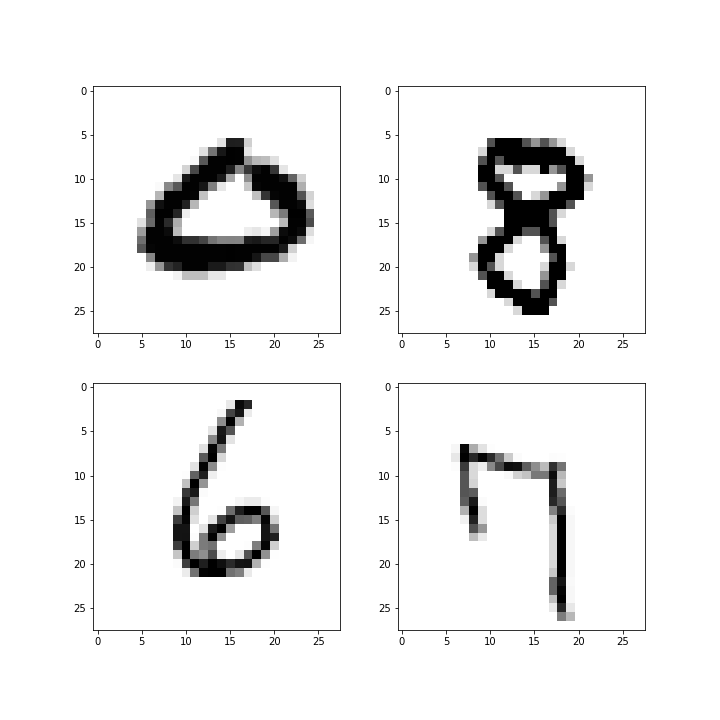
\includegraphics[width=1\linewidth]{MNISTExamples.png}
\end{subfigure}%
\begin{subfigure}{.6\textwidth}
  \centering
  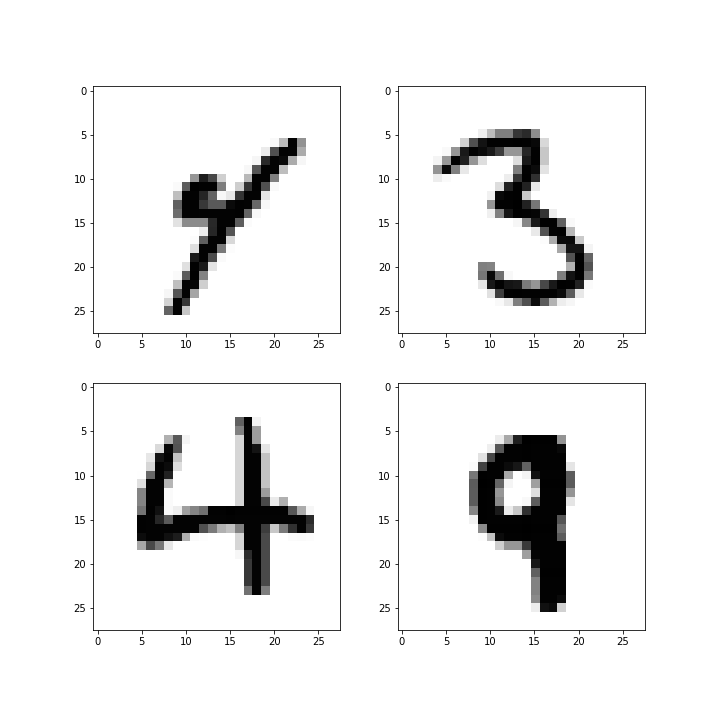
\includegraphics[width=1\linewidth]{MNISTExamples2.png}
\end{subfigure}
\caption{Sample figures from the MNIST dataset}
\label{fig:MNISTSamples}
\end{figure}
\subsection{CIFAR 10}\label{CIFAR10}
The CIFAR 10 dataset \cite{krizhevsky2009learning} is another image classification dataset; the inputs for each samples are 32x32x3 RGB colour pixel values (3 separate channels for the Red, Green and Blue colour value), while the labels specify the class of each image. The possible classes are `airplane', `automobile', `bird', `cat', `deer', `dog' ,'frog', `horse', `ship' and truck'. As can be seen in Figure \ref{fig:CIFARSamples}, the images are significantly downsampled, resulting in images that can be difficult even for a human observer to classify, resulting in a significantly more difficult task than either MNIST or the Geometric Shapes database. For this dataset we use convolutional networks, as introduced in Section \ref{sec:convnets}, this will both improve the results of the experiments with CIFAR 10, but will also test the performance of the curriculum methods with a different type of network.

\begin{figure}[h!]
\hspace*{-2cm}    
\centering
\begin{subfigure}{.6\textwidth}
  \centering
  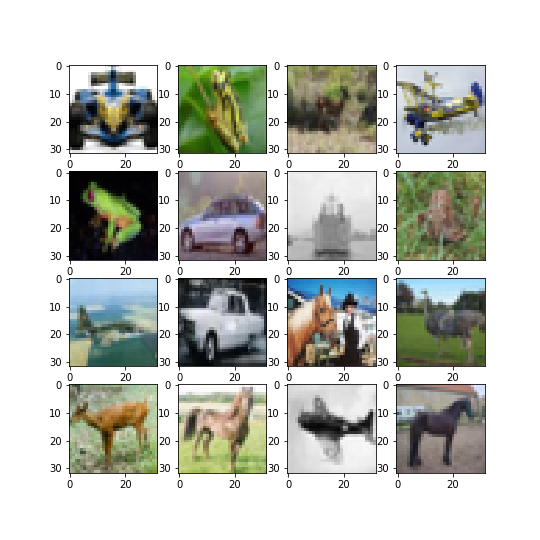
\includegraphics[width=1\linewidth]{CIFARExamples.png}
\end{subfigure}%
\begin{subfigure}{.6\textwidth}
  \centering
  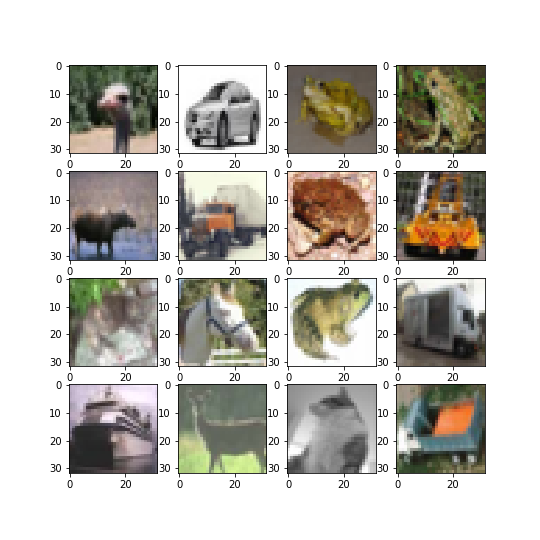
\includegraphics[width=1\linewidth]{CIFARExamples2.png}
\end{subfigure}
\caption{Sample figures from the CIFAR 10 dataset}
\label{fig:CIFARSamples}
\end{figure}



\section{Experiments}
We test the different dynamic curriculum methods introduced above on the Geometric Shapes, MNIST and CIFAR 10 image classification datasets, as introduced in Sections \ref{sec:GeoShapes}, \ref{MNIST} and \ref{CIFAR10}, respectively. For each dataset we used the validation set to construct an architecture and hyperparameters which achieved reasonable accuracies, then used those setting in the experiments for the different curriculum methods, the architectures for each dataset are laid out in Tables \ref{tab:GeoArchitecture2} to \ref{tab:CIFARArchitecture}. Note that in the case of CIFAR, the convolutional layer (denoted ``conv'') are following by a max pooling layer \cite{nagi2011max} and a batch normalization layer \cite{ioffe2015batch}, and ReLU denotes the Rectified Linear Unit activation function\cite{nair2010rectified}. 

\begin{table}[h!]
\caption{Geometric Shapes Dataset Model Architecture} \label{tab:GeoArchitecture2}
\begin{tabular}{|c||c|c|c|c|c|c|c|}
\hline
\multicolumn{8}{|c|}{Geometric Shapes Dataset Model Architecture} \\
\hline
 & Layer 1 & Layer 2 & Layer 3& Layer 4 &Layer 5 & Layer 6 & Layer 7 \\
\hline
\hline
Layer Type & FC & Dropout & FC & Dropout & FC & Dropout  & FC \\
\hline
Units & 300 & NA & 300 & NA & 300 & NA & 3 \\
\hline
Activation & Tanh & NA & Tanh & NA & Tanh & NA & Softmax \\
\hline
\end{tabular}
\end{table}

\begin{table}[h!]
\caption{MNIST Dataset Model Architecture} \label{tab:MNISTArchitecture}
\begin{tabular}{|c||c|c|c|c|c|c|c|}
\hline
\multicolumn{8}{|c|}{MNIST Dataset Model Architecture} \\
\hline
 & Layer 1 & Layer 2 & Layer 3& Layer 4 &Layer 5 & Layer 6 & Layer 7 \\
\hline
\hline
Layer Type & FC & Dropout & FC & Dropout & FC & Dropout  & FC \\
\hline
Units & 300 & NA & 300 & NA & 300 & NA & 3 \\
\hline
Activation & ReLU & NA & ReLU & NA & ReLU & NA & Softmax \\
\hline
\end{tabular}
\end{table}

\begin{table}[h!]
\caption{CIFAR Dataset Model Architecture} \label{tab:CIFARArchitecture}
\begin{tabular}{|c||c|c|c|c|c|c|c|}
\hline
\multicolumn{8}{|c|}{CIFAR Dataset Model Architecture} \\
\hline
 & Layer 1 & Layer 2 & Layer 3& Layer 4 &Layer 5 & Layer 6 & Layer 7 \\
\hline
\hline
Layer Type & Conv & Conv & Flatten & Dropout & FC & Dropout  & FC \\
\hline
Units & 50 & 50 & NA & NA & 100 & NA & 10 \\
\hline
Activation & ReLU &ReLU & NA & NA & ReLU & NA & Softmax \\
\hline
Kernel Size & 3x3 &3x3 & NA &NA &NA &NA &NA  \\
\hline
\end{tabular}
\end{table}

We run experiments across all three datasets using the curriculum methods laid out above, testing both `easy to hard' curricula and `hard to easy' curricula, as well as tested using different uncertainty functions. In each case we also train a baseline model with an equal number of epochs to provide a comparison for the curriculum test performance. We did not test all permutations of curricula and uncertainty functions as it became clear in early experiments some cases that there was little difference from the baseline performance, the experiments for which we performed repeated tests and presents present results are as follows:
\begin{itemize}
\item Geometric Shapes, using the AADT uncertainty function:
\begin{itemize}
\item{Dynamic Task Curriculum, Easy to Hard}
\item{Dynamic Task Curriculum, Hard to Easy}
\item{Dynamic Sampling Curriculum, Hard to Easy}
\item{Dynamic Sampled Task Curriculum, Hard to Easy}
\item{Uniform Sampling Baseline}
\end{itemize}
\item MNIST, using the AADT uncertainty function:
\begin{itemize}
\item{Dynamic Task Curriculum, Easy to Hard}
\item{Dynamic Sampling Curriculum, Easy to Hard}
\item{Dynamic Sampled Task Curriculum, Easy to Hard}
\item{Dynamic Task Curriculum, Hard to Easy}
\item{Dynamic Sampling Curriculum, Hard to Easy}
\item{Dynamic Sampled Task Curriculum, Hard to Easy}
\item{Uniform Sampling Baseline}
\end{itemize}
\item CIFAR 10, using the BALD uncertainty function\footnote {Tests for CIFAR 10 with the AADT function resulted in little difference with from baseline, however using the BALD uncertainty function improved performance significantly}:
\begin{itemize}
\item{Dynamic Task Curriculum, Easy to Hard}
\item{Dynamic Sampled Task Curriculum, Easy to Hard}
\item{Dynamic Task Curriculum, Hard to Easy}
\item{Dynamic Sampled Task Curriculum, Hard to Easy}
\item{Uniform Sampling Baseline}
\end{itemize}
\end{itemize}


We run the experiments 10 times with different random initialistions, reporting average results and standard errors. In Table \ref{tab:HyperParams2} we lay out the other hyperparameters for the experiments. Note that in each case we keep the number of tasks at 2, results were robust to differing the number of tasks however as we did not have time to do a full analysis we decided to keep the experimental setups relatively homogeneous in order to avoid tinkering with hyperparameters to achieve positive results. As in Chapter \ref{ch:BootstrappedActiveCurricula}, experiments were carried out in Keras \cite{chollet2015keras} and the Adam optimiser is implemented with the default hyperparameters (except for the learning rate which is given in Table \ref{tab:HyperParams2}). 

\begin{table}[h!]
\caption{Experiment Hyperparameters} \label{tab:HyperParams2}
\hspace*{-2cm}
\begin{tabular}{|c||c|c|c|c|c|c|c|}
\hline
\multicolumn{7}{|c|}{Experiment Hyperparameters} \\
\hline
 &Epochs & Optimiser &Learning Rate & Dropout \% & Batch Size & Num Tasks\\
\hline
Geometric Shapes & 350 & Adam & 0.0001 & 0.25 & 32 & 2  \\
\hline
MNIST & 50 & Adam & 0.0001 & 0.25 & 50 & 2  \\
\hline
CIFAR 10 & 50 & Adam & 0.0001 & 0.25 & 100 & 2  \\
\hline
\end{tabular}
\end{table}


\section{Results and Discussion}
The results for  the experiments are given in Tables \ref{tab:GeoShapes DACResults} to \ref{tab:CIFAR DACResults}\footnote{Due to the experimental setup for the CIFAR 10 experiments, only test accuracies were recorded.}, and illustrated in Figures \ref{fig:GeoShapesDACResults} and \ref{fig:DACResults}. Note that the denotation `easy' implies that the curriculum was trained on an easy-hard curriculum, with increasingly difficult tasks in the DTC case and by biasing sampling towards easy samples in the DSC method, and similarly for the DSTC method. Conversely, `Hard' denotes that the curriculum used was a hard to easy curriculum.
\begin{table}[h!]
\caption{Geometric Shapes DAC Results} \label{tab:GeoShapes DACResults}
\begin{tabular}{|c||c|c|}
\hline
\multicolumn{3}{|c|}{GeoShapes DAC Results} \\
\hline
 & Test Accuracy (\%) & Test Cross-Entropy Error \\
\hline
Uniform Baseline&  0.826 $\pm$ 0.00281 & 0.437 $\pm$ 0.00696 \\
\hline
DSC - Hard& 0.846$ \pm$ 0.00369 & 0.391 $\pm$ 0.00827 \\
\hline
DTC - Hard&  0.865  $\pm$ 0.00157 & 0.362 $\pm$ 0.00350 \\
\hline
DSTC - Hard & 0.866 $\pm$ 0.00192 & 0.355 $\pm$ 0.00502 \\
\hline
DTC - Easy & 0.830 $\pm$ 0.00198 & 0.420 $\pm$ 0.00469 \\
\hline
\end{tabular}
\end{table}

\begin{table}[h!]
\caption{MNISTShapes DAC Results} \label{tab:MNIST DACResults}
\begin{tabular}{|c||c|c|}
\hline
\multicolumn{3}{|c|}{MNIST DAC Results} \\
\hline
 & Test Accuracy (\%) & Test Cross-Entropy Error \\
\hline
Uniform Baseline&  0.975 $\pm$ 0.000188& 0.229 $\pm$ 0.000562 \\
\hline
DSC - Hard& 0.977$ \pm$ 0.000216& 0.250 $\pm$ 0.000497 \\
\hline
DTC - Hard&  0.977  $\pm$ 0.000216 & 0.227 $\pm$ 0.000611 \\
\hline
DSTC - Hard & 0.979 $\pm$ 0.000327 & 0.251 $\pm$ 0.000736\\
\hline
DSC - Easy& 0.970$ \pm$ 0.000240 & 0.227 $\pm$ 0.00102 \\
\hline
DTC - Easy & 0.970 $\pm$ 0.000276 & 0.224 $\pm$ 0.000696 \\
\hline
DSTC - Easy & 0.964 $\pm$ 0.000314 & 0.228$\pm$ 0.000595 \\
\hline
\end{tabular}
\end{table}

\begin{table}[h!]
\caption{CIFAR 10 DAC Results} \label{tab:CIFAR DACResults}
\begin{tabular}{|c||c|}
\hline
\multicolumn{2}{|c|}{CIFAR 10 DAC Results} \\
\hline
 & Test Accuracy (\%) \\
\hline
Uniform Baseline&  0.713 $\pm$ 0.00439\\
\hline
DTC - Hard&  0.730 $\pm$ 0.00132 \\
\hline
DSTC - Hard & 0.725 $\pm$ 0.00129\\
\hline
DTC - Easy & 0.727 $\pm$ 0.00197 \\
\hline
DSTC - Easy & 0.722 $\pm$ 0.00429 \\
\hline
\end{tabular}
\end{table}



\begin{figure}[h!]
\hspace*{-3cm}    
\centering
\begin{subfigure}{0.7\textwidth}
  \centering
  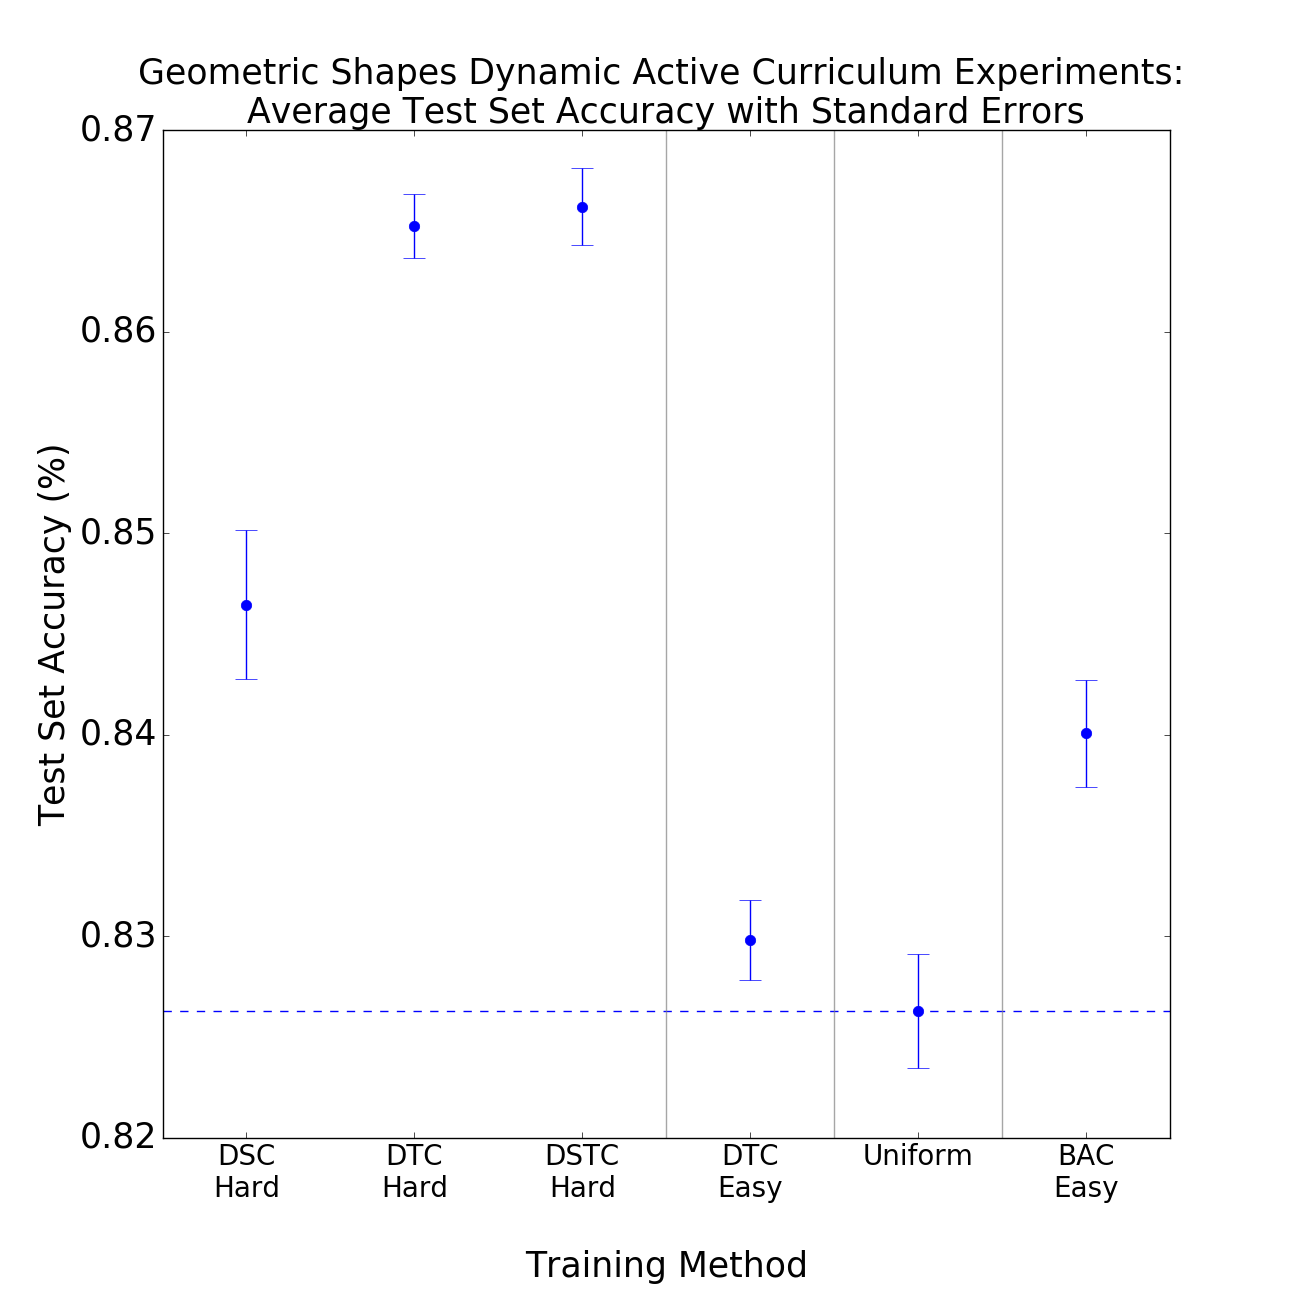
\includegraphics[width=1\linewidth]{GeoShapes_Dynamic_Results_STE.png}
  \caption{ Mean Test Set Accuracies}
  \label{fig:DAC_ste_Geo}
\end{subfigure}%
\begin{subfigure}{0.7\textwidth}
\hspace*{-1cm}   
  \centering
  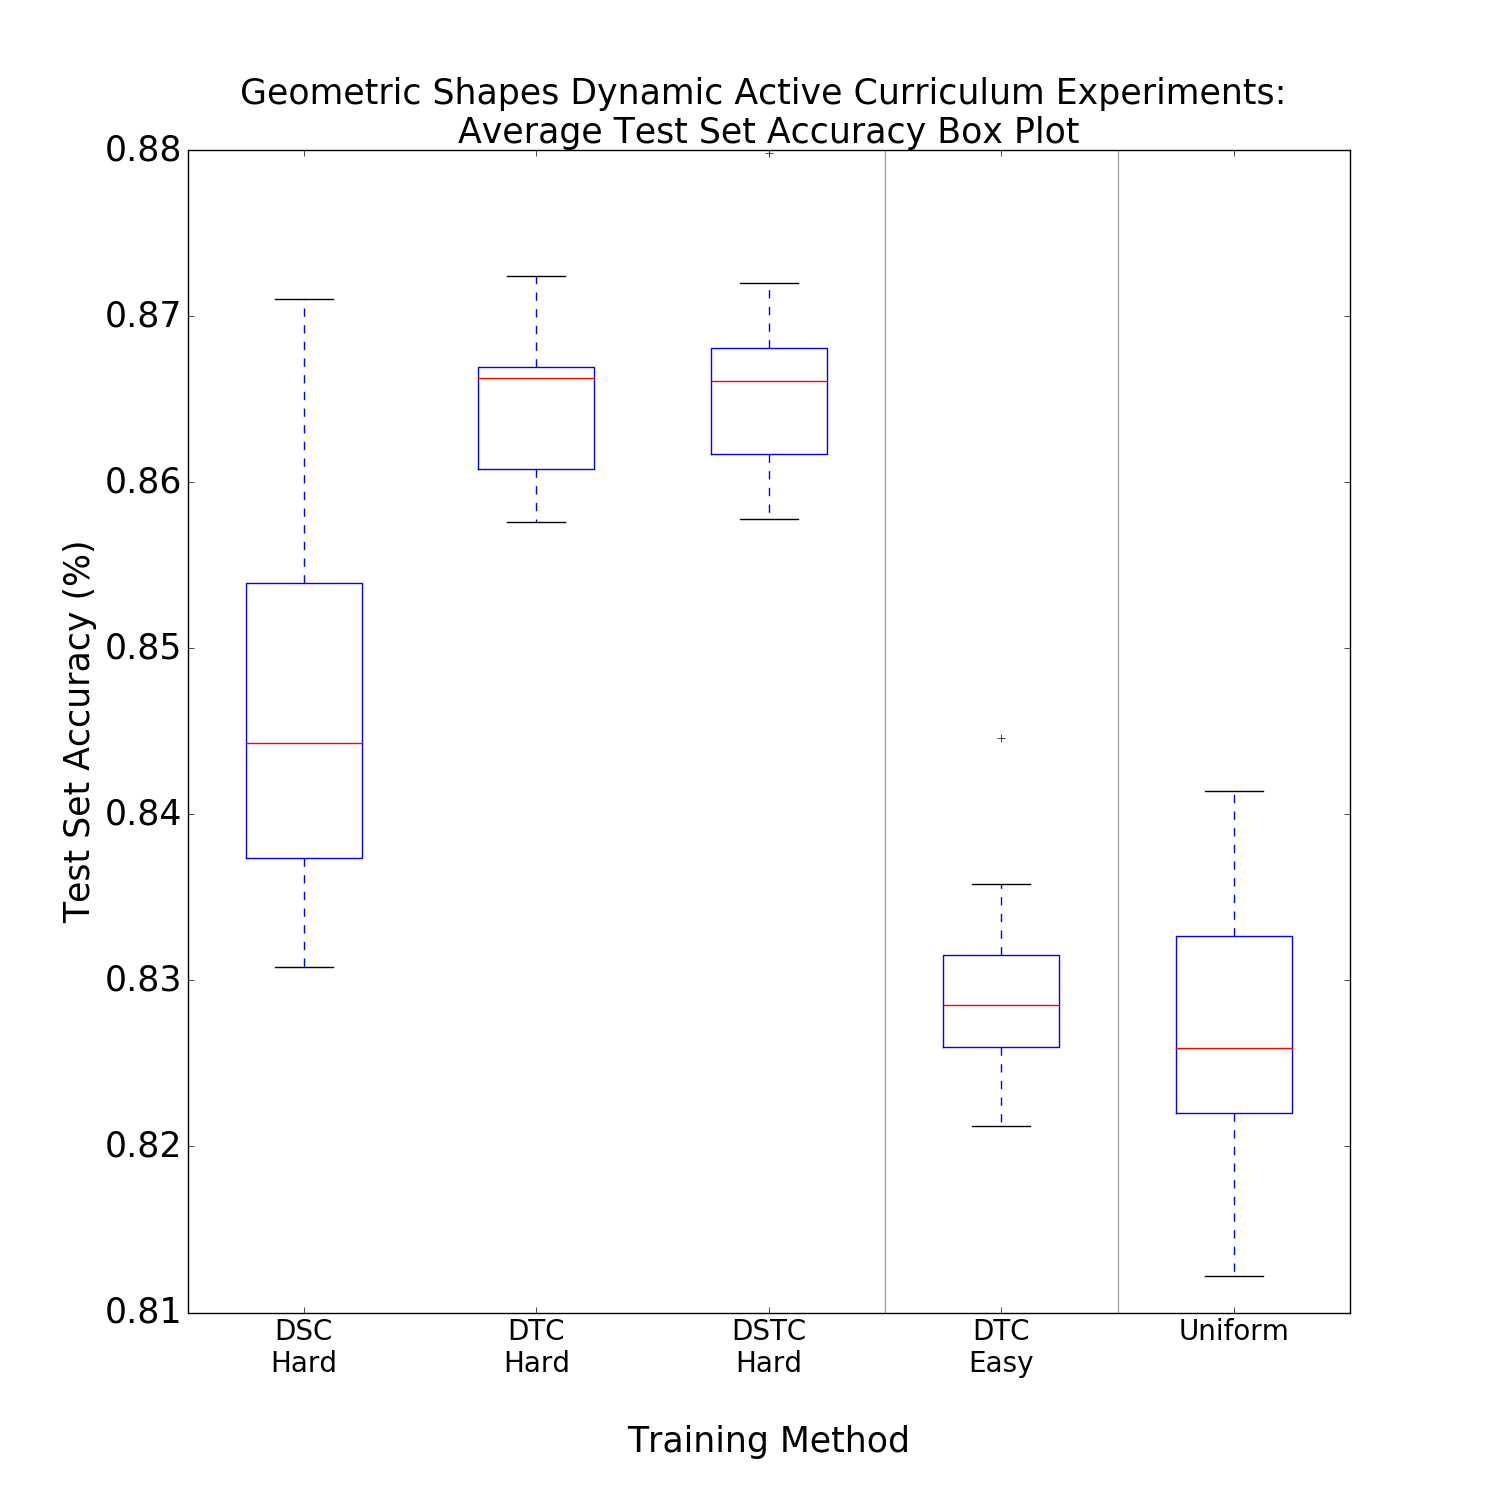
\includegraphics[width=1\linewidth]{GeoShapes_Dynamic_Results_Boxplt.png}
  \caption{Test Set Accuracy Boxplots}
  \label{fig:DAC_BoxPlt_Geo}
\end{subfigure}
\caption{Geometric Shapes Dynamic Active Curriculum (DAC) Experiment Results}
\label{fig:GeoShapesDACResults}
\end{figure}

\begin{figure}[h!]
\hspace*{-3cm}    
\centering
\begin{subfigure}{0.7\textwidth}
  \centering
  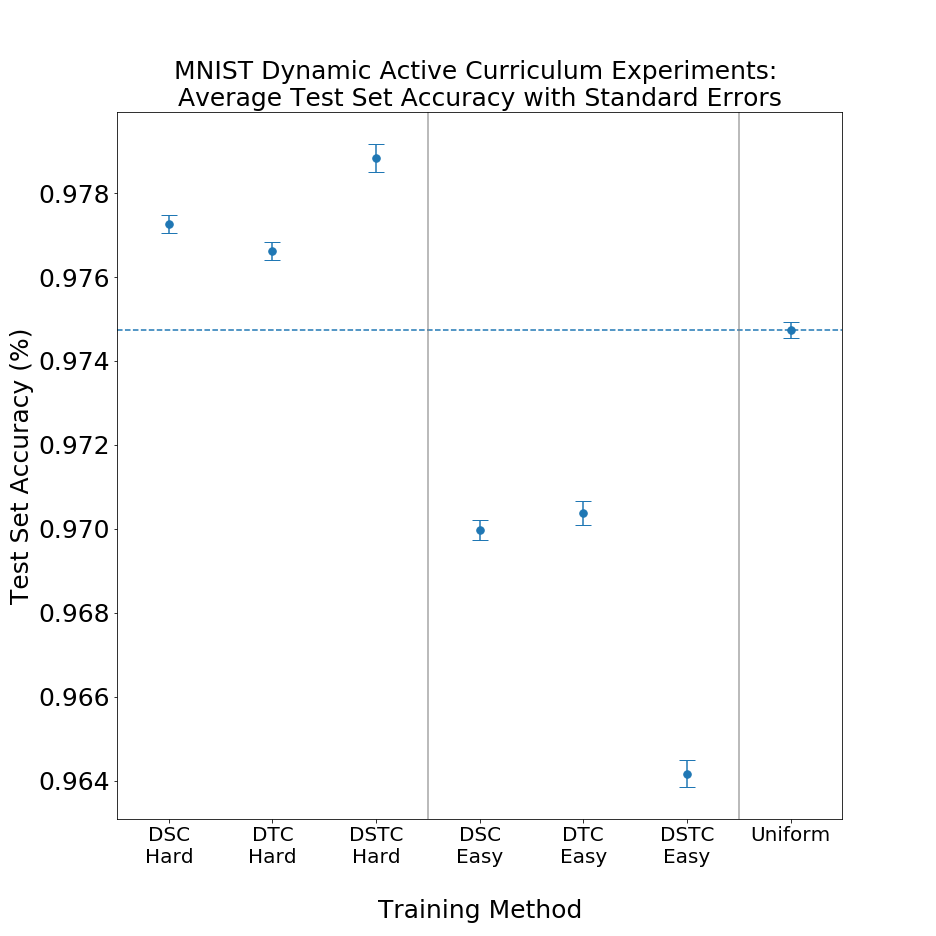
\includegraphics[width=1\linewidth]{MNIST_Dynamic_Results.png}
  \caption{ Mean Test Set Accuracies}
  \label{fig:DAC_ste_MNIST}
\end{subfigure}%
\begin{subfigure}{0.7\textwidth}
\hspace*{-1cm}   
  \centering
  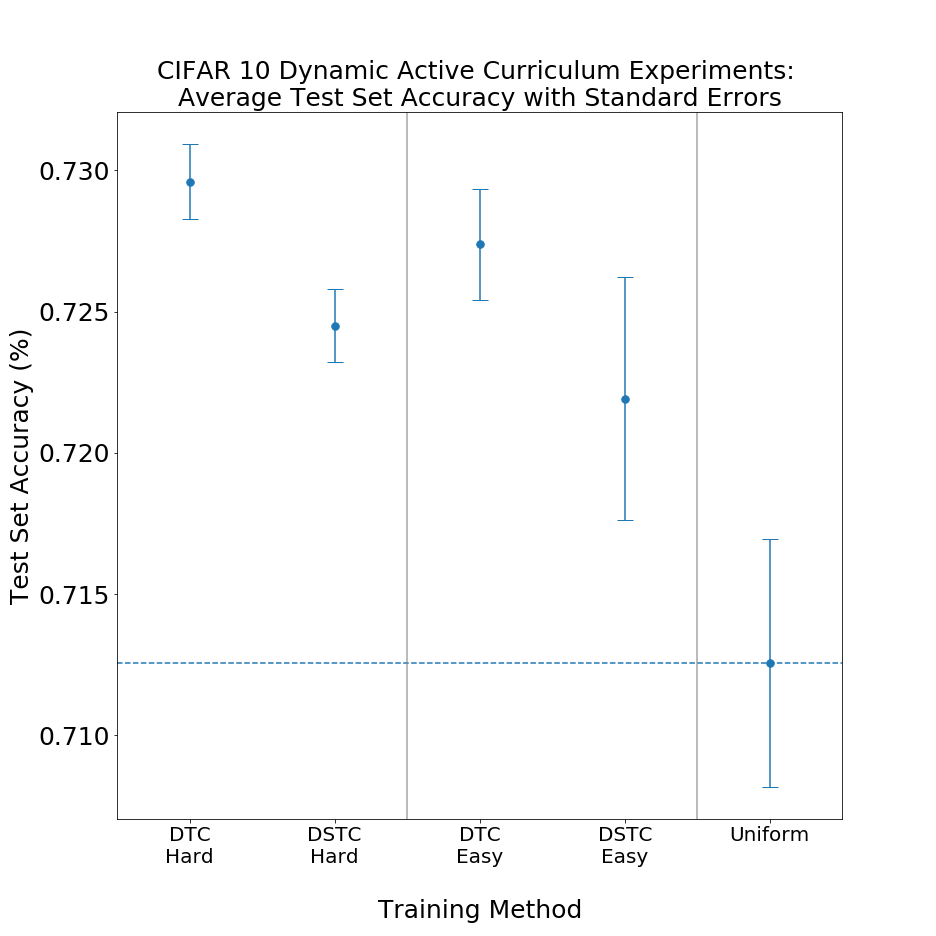
\includegraphics[width=1\linewidth]{CIFAR_Dynamic_Results.png}
  \caption{Test Set Accuracy Boxplots}
  \label{fig:DAC_ste_CIFAR}
\end{subfigure}
\caption{MNIST and CIFAR 10 Dynamic Active Curriculum (DAC) Experiment Results}
\label{fig:DACResults}
\end{figure}